%----------------------------------------------------------------------------
\chapter{Sample application}
%----------------------------------------------------------------------------

This chapter presents the design and implementation of the sample application which will act as a case-study to showcase the features of the test framework and to serve as a basis for future enhancements. 


%----------------------------------------------------------------------------
\section{Design}
%----------------------------------------------------------------------------

%----------------------------------------------------------------------------
\subsection{Requirements} \label{sample-app-requirements}
%----------------------------------------------------------------------------

%\begin{itemize}
%	\item objectives
%	\begin{itemize}
%		\item microservices architecture
%		\item containerization - facilitates easy deployment and scalability
%		\item have a system with different components based on state-fullness (stateful, stateless, )
%		\item have component(s) that can be scaled based on some application specific workload requirements (e.g. increased load on the system, fault tolerant redundancy) - stateless components can be scaled more easily
%		\item observable and collectible application specific metrics
%	\end{itemize}
%\end{itemize}

The design of the sample application was driven by several requirements to create a system that can be easily used for our purposes.

\paragraph{Kubernetes ready}The purpose of the thesis is to inspect dependability metrics in Kubernetes environments, this naturally means that the application should be able to run on a Kubernetes cluster.

\paragraph{Microservices architecture}As the application needs to be deployed and function in a Kubernetes-based environment, it was evident that a microservice architecture was the right choice for starting the design of the system. This notion implicitly means that there will be multiple, independent components that have to communicate with each other in order to create a whole system.

\paragraph{Scalability}In a real world application it is quite important to create systems that by design can handle different amount of workloads without any major impact on user experience. At the same, an economic use of resources is also a significant requirement, so the system does not reserve too much resources and keeps them idle(\eg CPU, memory, storage, network bandwidth). That means the system should be able to dynamically change and fine tune its capacity and performance to satisfy both constraints. In addition, the application specific triggers for scaling should also be clearly defined.

\paragraph{Containerization}The ease of deployment and scalability is one of the cardinal goals of designing and maintaining a microservice application. Containerization provides the fundamentals for achieving this as all the dependencies and configuration needed for a component can be placed in a container. This leads to the conclusion that each component should be packaged and deployed into separate and independent containers.  In terms of scalability this form of packaging and deployment enables horizontal scaling, that means \eg during a bigger system usage, more instances of a given components should be started instead of increasing the resources of a single component instance.

\paragraph{Stateful and stateless components}The aim of the sample application is to attempt to provide a fair generalization of different kind of system components. A popular classification is deciding whether a component is stateful or stateless. This characteristic greatly affects how a given is able to scale as stateless components are usually easier to manage in terms of scalability. To have the possibility of showcasing the scenario of scaling both types of components, there should be both stateful and stateless components in the case study system.

\paragraph{Observable application metrics}In order to be able to reason about the dependability and performance of the system, different kind of numerical metrics should be available to evaluate. This poses the requirement to create a system that can be easily monitored. The 
components should provide an interface that other tools can use to collect metrics describing both application specific behavior and the state of underlying layers (\eg CPU usage, memory usage, network communication).


%----------------------------------------------------------------------------
\subsection{Architecture}
%----------------------------------------------------------------------------

Although the aim of the sample application is to attempt to provide a generalized system to fit many use-cases without limiting possibilities, when it comes to architectural design, it is indispensable to create the structure of the system with a specific use-case in mind. But with a fairly common use case, the fundamental goal can be roughly preserved.

For this project, a master-worker architecture was chosen, where the master component receives input from clients and then assigns computational tasks to the workers based on the parameters. This architecture allows to easily define scalable, and both stateful and stateless components. The abstract workflow of the use case is the following:

TODO: activity diagram?

\begin{enumerate}
	\item \emph{Submit tasks } A client submits input parameters to the master component.
	\item \emph{Distribute tasks} The master component creates a task definition based on the input parameters and then forwards it to one of the worker components.
	\item \emph{Task execution} The worker components executes the received task and sends back the result to the master.
	\item \emph{Persist results} The master persists the result of the completed task.
\end{enumerate}

The designed architecture of the sample application can be seen in Figure \ref{fig:sample_app_arch}

\begin{figure}[h]
	\centering
	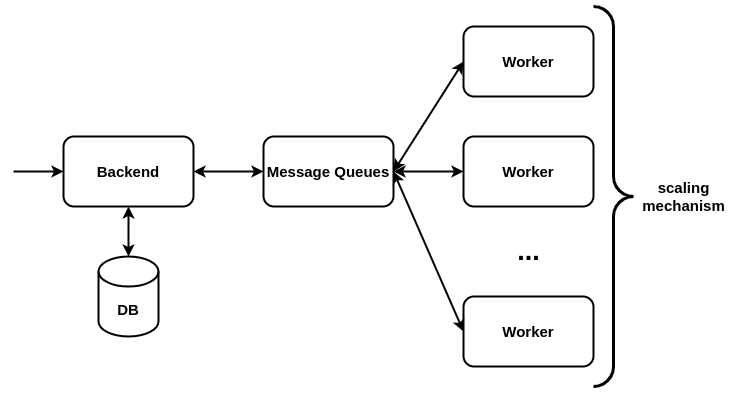
\includegraphics[width=130mm, keepaspectratio]{figures/sample_app_arch.png}
	\caption{Sample application architecture}
	\label{fig:sample_app_arch}
\end{figure}

%----------------------------------------------------------------------------
\subsection{Communication}
%----------------------------------------------------------------------------

Before commencing with the design of each component, it is important to specify how the components in the system will communicate with each other as this can affect their construction. Considering that the sample application tries to resemble implementations that are widely used in the industry, the components to be created in this project will expose REST API endpoints and will communicate over HTTP protocol. This provides the right degree of customizability on the component level while allowing loose-coupling on the system level. 


%\begin{itemize}
%	\item master-worker architecture
%	\item REST API interfaces
%	\item use-case
%	\begin{itemize}
%		\item submitting computation jobs
%		\item distributing jobs among worker nodes
%		\item persisting job results
%		\item querying job results
%	\end{itemize}
%	
%\end{itemize}


%----------------------------------------------------------------------------
\subsection{Components}
%----------------------------------------------------------------------------

In the following sections, each component and their responsibilities are presented.

%----------------------------------------------------------------------------
\subsubsection{Backend}
%----------------------------------------------------------------------------

\begin{itemize}
	\item provides a REST API interface for submitting new jobs and querying their result
	\item forward submitted jobs to worker nodes
	\item stores the result of finished jobs in a database
	\item exposes a metrics endpoint for external monitoring solutions
	\item exposes health endpoint that can be consumed to verify that the system works in a functionally correct way
\end{itemize}

responsibilites + API + health endpoint

%----------------------------------------------------------------------------
\subsubsection{Worker}
%----------------------------------------------------------------------------

\begin{itemize}
	\item provides a REST API interface to accept jobs from the backend to execute
	\item exposes a metrics endpoint for external monitoring solutions
	\item exposes health endpoint
\end{itemize}

responsibilites + API + health endpoint

%----------------------------------------------------------------------------
\subsubsection{Message Queue}
%----------------------------------------------------------------------------

\begin{itemize}
	\item connects the backend with the worker nodes
	\item as the number of worker nodes is dynamic, it would be not feasible for the backend to try to keep record of all the running workers
	\item the backend sends the jobs to the workers via this message queue
	\item the the workers also use this to send back the finished jobs (at the moment, we could skip the message queue on the way back, but this way we do not need much modification if there would be more than one backend in order to \eg be able to handle a bigger load)
\end{itemize}

%----------------------------------------------------------------------------
\subsubsection{Database}
%----------------------------------------------------------------------------

\begin{itemize}
	\item stores the jobs with their result 
	\item serves queries made by the backend component
\end{itemize}

%----------------------------------------------------------------------------
\section{Implementation}
%----------------------------------------------------------------------------

\begin{itemize}
	\item Introduce the general problem it solves (naive implementation of Fibonacci - this is implementation)
	\item Docker
\end{itemize}

%----------------------------------------------------------------------------
\subsection{Backend}
%----------------------------------------------------------------------------

\begin{itemize}
	\item Spring Boot Java
	\item introduce Job model
	\item introduce REST API
	\item introduce health check
	\item introduce Message Queue integration
\end{itemize}

%----------------------------------------------------------------------------
\subsection{Worker}
%----------------------------------------------------------------------------

\begin{itemize}
	\item Spring Boot Java
	\item introduce REST API
	\item introduce health check
	\item introduce Message Queue integration
\end{itemize}

%----------------------------------------------------------------------------
\subsection{Message Queue}
%----------------------------------------------------------------------------

\begin{itemize}
	\item configuration? image?
\end{itemize}

%----------------------------------------------------------------------------
\subsection{Database}
%----------------------------------------------------------------------------

\begin{itemize}
	\item configuration? image?
\end{itemize}


\subsection{Kubernetes definitions}


\begin{itemize}
	\item K8s pod, depl, svc exapmle (one for each)
	\item HPA definition, metrics server
\end{itemize}
















